\documentclass[a4paper,11pt,notitlepage,fullpage]{article}
%\documentclass{report}

\usepackage{fullpage}
\usepackage[utf8]{inputenc}
%\usepackage[ngerman]{babel}
%\usepackage[english]{babel}
\usepackage{amsmath}
\usepackage{amssymb}
\usepackage{latexsym}
\usepackage{mathtools}
\usepackage{listings}
\usepackage{bbm}
%\usepackage{algorithm}
%\usepackage{algpseudocode}
\usepackage{graphicx}
\usepackage{booktabs}
\usepackage{hhline}
\usepackage{amsthm}
\usepackage{cite}
\usepackage{wrapfig}
\usepackage{hyperref}
\usepackage{titling}
\usepackage{color}

\setlength{\droptitle}{-60pt}

\newcommand{\R}{\mathbb R}
\newcommand{\N}{\mathbb N}

\newcommand{\p}{\mathbb P}
\newcommand{\pp}[1]{\mathbb P\left[#1\right]}
\newcommand{\E}{\mathbb E}
\newcommand{\Ee}[1]{\mathbb E\left[#1\right]}
\newcommand{\V}{\mathbb V}
\newcommand{\Vv}[1]{\mathbb V\left[#1\right]}
\newcommand{\Cov}[1]{\mathbb Cov\left[#1\right]}
\newcommand{\F}{\mathcal{F}}
\newcommand{\ind}{\mathbbm{1}}
\newcommand{\indd}[1]{\mathbbm{1}_{#1}}
\newcommand{\norm}[2]{\left|\left|{#1}\right|\right|_{#2}}

\begin{document}
\author{Florian Bogner \& Alexander Palmrich}
\title{Stochastische Prozesse - Übung 5}
\maketitle

\begin{enumerate}
\setcounter{enumi}{20}

%21
\item Sei 
\begin{align*}
f(t) &:= W(t) \indd{[0,1)}(t)\\
f_n(t) &:= \sum_{j=0}^{n-1} W(\frac{j}{n}) \indd{[\frac{j}{n}, \frac{j+1}{n})}(t)\\
Y &:= \frac{W(1)^2-1}{2}
\end{align*}

\begin{figure}[h!]
\centering
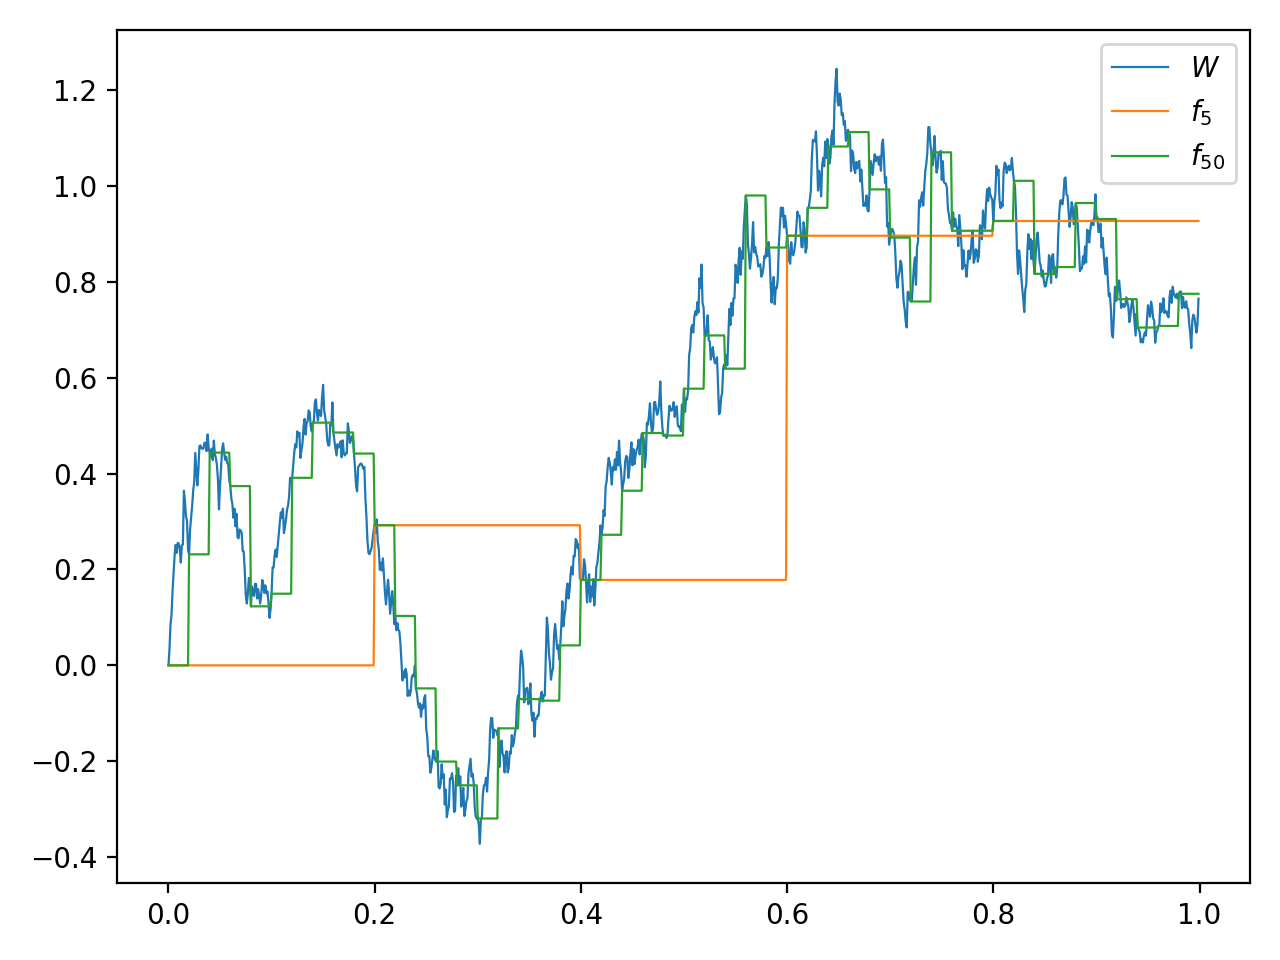
\includegraphics[width=0.9\textwidth]{gfx/21_fig.png}
\caption{Ein typischer Pfad von $W$, $f$ und $f_n$}
\end{figure}

\begin{enumerate}
%a
\item $M^2$-Fehler der Approximation von $f$ bestimmen.
\begin{align*}
\norm{f_n-f}{M^2} &= \norm{\sum_{j=0}^{n-1} \left(W(\frac{j}{n})-W(t)\right) \indd{[\frac{j}{n}, \frac{j+1}{n})}(t)}{M^2}\\
&= \Ee{\int \sum_{j=0}^{n-1} \left(W(\frac{j}{n})-W(t)\right)^2 \indd{[\frac{j}{n}, \frac{j+1}{n})}(t) dt}\\
&= \int \Ee{\sum_{j=0}^{n-1} \left(W(\frac{j}{n})-W(t)\right)^2 \indd{[\frac{j}{n}, \frac{j+1}{n})}(t) } dt &\text{(Fubini-Tonelli)}\\
&= \int \sum_{j=0}^{n-1} \Ee{\left(W(\frac{j}{n})-W(t)\right)^2} \indd{[\frac{j}{n}, \frac{j+1}{n})}(t)  dt\\
&= \int \sum_{j=0}^{n-1} \left(t-\frac{j}{n}\right) \indd{[\frac{j}{n}, \frac{j+1}{n})}(t)  dt & \text{($W$ neu gestartet)}\\
&=  \sum_{j=0}^{n-1} \int\left(t-\frac{j}{n}\right) \indd{[\frac{j}{n}, \frac{j+1}{n})}(t)  dt \\
&=  \sum_{j=0}^{n-1} \frac{1}{2n^2} & \text{($\int$ = halbes Quadrat der Länge $\frac{1}{n}$)}\\
&= \frac{1}{2n}
\end{align*}
Man beachte, dass mit Itô-Isometrie gilt
$$\frac{1}{2n} = \norm{f_n-f}{M^2} = \norm{I(f_n-f)}{L^2} = \norm{I(f_n)-I(f)}{L^2} = \norm{I(f_n)-Y}{L^2}$$

%b
\item $L^2$-Fehler der Approximation der Itô-Integrale, ohne Isometrie.
\begin{align*}
\norm{I(f_n)-Y}{L^2} = ?
\end{align*}
\end{enumerate}


%22
\item Sei
$$g_n(t) := \sum_{j=0}^{n-1} (W(\frac{j}{n}))^2 \indd{[\frac{j}{n}, \frac{j+1}{n})}(t)$$
\begin{enumerate}
%a
\item Varianz des Itô-Integrals ausrechnen.
\begin{align*}
\Vv{I(g_n)} &= \Ee{(I(g_n))^2}\\
&=\Ee{\int g_n^2 dt}\\
&= \int \Ee{g_n^2} dt\\
&= \int \Ee{\sum_{j=0}^{n-1} (W(\frac{j}{n}))^4 \indd{[\frac{j}{n}, \frac{j+1}{n})}(t)} dt\\
&= \int \sum_{j=0}^{n-1} \Ee{(W(\frac{j}{n}))^4} \indd{[\frac{j}{n}, \frac{j+1}{n})}(t) dt\\
&= \int \sum_{j=0}^{n-1} 3(\frac{j}{n})^4 \indd{[\frac{j}{n}, \frac{j+1}{n})}(t) dt\\
&= \sum_{j=0}^{n-1} 3(\frac{j}{n})^4 \int \indd{[\frac{j}{n}, \frac{j+1}{n})}(t) dt\\
&= \sum_{j=0}^{n-1} 3(\frac{j}{n})^4 \frac{1}{n}\\
&= \frac{3}{n^5} \sum_{j=0}^{n-1} j^4 \\
\end{align*}

%b
\item Summen über eine feste Potenz natürlicher Zahlen: Nach wem sind Formeln benannt, die sowas anders darstellen?
\begin{align*}
\end{align*}
\end{enumerate}

%23
\item Markovkette mit vier Zuständen, Anfangsverteilung $\lambda = (0.5, 0.5, 0, 0)$ und der Übergangsmatrix
$$P=\begin{pmatrix}
\frac{1}{3} & \frac{1}{3} & 0 & \frac{1}{3} \\
\frac{1}{4} & \frac{1}{4} & \frac{1}{4} & \frac{1}{4} \\
0 & 0 & \frac{1}{2} & \frac{1}{2} \\
0 & 0 & 0 & 1
\end{pmatrix}$$
\begin{enumerate}
%a
\item Wir verwenden das Prinzip $\pp{A \wedge B} = \pp{A} \cdot \pp{B|A}$. Wegen der Markoveigenschaft können wir die gesamte Bedingung auf die Bedingung durch den letzten Zeitpunkt runterbrechen. Damit ergibt sich:
\begin{align*}
&\pp{X_0 = 2, X_1 = 1, X_2 = 2, X_3 = 1} \\
=~&\pp{X_0 = 2} \cdot \pp{X_1 = 1 | X_0 = 2} \cdot \pp{X_2 = 2 | X_1 = 1} \cdot \pp{X_3 = 1 | X_2 = 2} \\
=~&\lambda_2 \cdot P_{2, 1} \cdot P_{1, 2} \cdot P_{2, 1} \\
=~&\frac{1}{2} \cdot \frac{1}{4} \cdot \frac{1}{3} \cdot \frac{1}{4} = \frac{1}{96}
\end{align*}
Desweiteren:
\begin{align*}
&\pp{X_0 = 2, X_2 = 2, X_3 = 1} \\
=~&\pp{X_0 = 2} \cdot \pp{X_2 = 2 | X_0 = 2} \cdot \pp{X_3 = 1 | X_2 = 2} \\
=~&\lambda_2 \cdot P^2_{2, 2} \cdot P_{2, 1} \\
=~&\frac{1}{2} \cdot (\frac{1}{3}\frac{1}{4} + \frac{1}{4}\frac{1}{4} + 0 \frac{1}{4}+ 0 \frac{1}{4}) \cdot \frac{1}{4} \\
=~&\frac{1}{2} \cdot \frac{7}{48} \cdot \frac{1}{4}  = \frac{7}{384}\\
\end{align*}

%b
\item Die Kommunikationsklassen sind $\{1, 2\}, \{3\}$ und $\{4\}$. Die ersten Beiden sind transient, die letzte ist rekurrent.

%c
\item Sei $T$ die Stoppzeit um in 1 oder 4 zukommen.
\begin{align*}
\end{align*}

%d
\item Mittlere Trefferzeit wie oben aber bei Start in jeweiligen Zuständen ausrechnen.
\begin{align*}
\end{align*}

%e
\item Varianz der Trefferzeit wie oben bei Start in $3$ ausrechnen.
\begin{align*}
\end{align*}
\end{enumerate}

%24
\item Marovkette mit fünf Zuständen, Übergangswahrscheinlichkeiten siehe Graph.
\begin{enumerate}
%a
\item Wahrscheinlichkeiten von zwei konkreten Zustandsfolgen ausrechnen.
\begin{align*}
\end{align*}

%b
\item Kette irreduzibel?
\begin{align*}
\end{align*}

%c
\item Trefferzeiten für $0$ endlich mit welcher $\p$?
\begin{align*}
\end{align*}

%d
\item LGS für mittlere Trefferzeiten in $0$ aufstellen.
\begin{align*}
\end{align*}
\end{enumerate}

%25
\item Wir spielen ein Münzwurfspiel um Geld, bei dem in jeder Runde unser Kapital um $\pm 1$ je nach Kopf/Zahl verändert wird. Was ist die Wahrscheinlichkeit, bei Startkapital $i$ in endlicher Zeit in den Ruin zu kommen? Wir bedienen uns einer Markovkette und dem zugehörigen LGS.

Für alle $a \in \R$ ist $(h_i := ai + 1)_{i \in \N}$ eine Lösung des LGS:
\begin{align*}
1 &\stackrel{!}{=} h_0 = a\cdot 0 + 1 = 1 \\
h_i &\stackrel{!}{=} \frac{1}{2}h_{i-1} + \frac{1}{2}h_{h+1} \\
&= \frac{1}{2}(a(i-1) + 1 + a(i+1) + 1)) \\
&= \frac{1}{2}(2ai + 2) \\
&= ai+1 = h_i
\end{align*}
Damit haben wir unendlich viele Lösungen. Das sind auch schon alle, denn $h_0 = 1$ ist fest, und $a := h_1 - 1$ berechnet sich aus $h_1$. Höhere $h_i$ für $i>1$ sind dann durch Induktion und die zweite Gleichung eindeutig bestimmt.

Für $a < 0$ ergeben sich $h_i < 0$ für große $i$\footnote{Jargon-Warnung: Weil $\R$ ein archimedischer Körper ist.}, also kann $h_i$ wohl keine Wahrscheinlichkeit sein. Analog, für $a > 0$ ist $h_1 > 1$, also kann es auch keine Wahrscheinlichkeit sein. Nur $a = 0$ und damit $h_i = 1$ bleibt als Möglichkeit übrig.

\end{enumerate}












\end{document}
